\documentclass[a4paper]{book}
\usepackage{makeidx}
\usepackage{graphicx}
\usepackage{multicol}
\usepackage{float}
\usepackage{listings}
\usepackage{color}
\usepackage{ifthen}
\usepackage[table]{xcolor}
\usepackage{textcomp}
\usepackage{alltt}
\usepackage{ifpdf}
\ifpdf
\usepackage[pdftex,
            pagebackref=true,
            colorlinks=true,
            linkcolor=blue,
            unicode
           ]{hyperref}
\else
\usepackage[ps2pdf,
            pagebackref=true,
            colorlinks=true,
            linkcolor=blue,
            unicode
           ]{hyperref}
\usepackage{pspicture}
\fi
\usepackage[utf8]{inputenc}
\usepackage{mathptmx}
\usepackage[scaled=.90]{helvet}
\usepackage{courier}
\usepackage{doxygen}
\lstset{language=C++,inputencoding=utf8,basicstyle=\footnotesize,breaklines=true,breakatwhitespace=true,tabsize=5,numbers=left }
\makeindex
\setcounter{tocdepth}{3}
\renewcommand{\footrulewidth}{0.4pt}
\begin{document}
\hypersetup{pageanchor=false}
\begin{titlepage}
\vspace*{7cm}
\begin{center}
{\Large Mbica \\[1ex]\large 1.0 }\\
\vspace*{1cm}
{\large Generated by Doxygen 1.7.3}\\
\vspace*{0.5cm}
{\small Wed Jan 25 2012 00:22:25}\\
\end{center}
\end{titlepage}
\clearemptydoublepage
\pagenumbering{roman}
\tableofcontents
\clearemptydoublepage
\pagenumbering{arabic}
\hypersetup{pageanchor=true}
\chapter{Namespace Index}
\section{Namespace List}
Here is a list of all namespaces with brief descriptions:\begin{DoxyCompactList}
\item\contentsline{section}{\hyperlink{namespacembica}{mbica} }{\pageref{namespacembica}}{}
\item\contentsline{section}{\hyperlink{namespacembica_1_1def}{mbica::def} (Default values for epsilon, max iterations and mu )}{\pageref{namespacembica_1_1def}}{}
\item\contentsline{section}{\hyperlink{namespacembica_1_1nonlinearities}{mbica::nonlinearities} }{\pageref{namespacembica_1_1nonlinearities}}{}
\end{DoxyCompactList}

\chapter{Class Index}
\section{Class Hierarchy}
This inheritance list is sorted roughly, but not completely, alphabetically:\begin{DoxyCompactList}
\item \contentsline{section}{mbica::FastICA\_\-impl}{\pageref{classmbica_1_1_fast_i_c_a__impl}}{}
\begin{DoxyCompactList}
\item \contentsline{section}{mbica::FastICA$<$ UsedNonl, Stabilization $>$}{\pageref{classmbica_1_1_fast_i_c_a}}{}
\end{DoxyCompactList}
\item \contentsline{section}{mbica::ICASeparator}{\pageref{classmbica_1_1_i_c_a_separator}}{}
\item \contentsline{section}{mbica::nonlinearities::Nonlinearity}{\pageref{classmbica_1_1nonlinearities_1_1_nonlinearity}}{}
\begin{DoxyCompactList}
\item \contentsline{section}{mbica::nonlinearities::Gauss$<$ a, b $>$}{\pageref{classmbica_1_1nonlinearities_1_1_gauss}}{}
\item \contentsline{section}{mbica::nonlinearities::Pow$<$ a $>$}{\pageref{classmbica_1_1nonlinearities_1_1_pow}}{}
\item \contentsline{section}{mbica::nonlinearities::TanH$<$ a, b $>$}{\pageref{classmbica_1_1nonlinearities_1_1_tan_h}}{}
\end{DoxyCompactList}
\item \contentsline{section}{mbica::NoStabilization}{\pageref{classmbica_1_1_no_stabilization}}{}
\item \contentsline{section}{mbica::PCA}{\pageref{classmbica_1_1_p_c_a}}{}
\item \contentsline{section}{mbica::Whitening}{\pageref{classmbica_1_1_whitening}}{}
\item \contentsline{section}{mbica::WithStabilization}{\pageref{classmbica_1_1_with_stabilization}}{}
\end{DoxyCompactList}

\chapter{Class Index}
\section{Class List}
Here are the classes, structs, unions and interfaces with brief descriptions:\begin{DoxyCompactList}
\item\contentsline{section}{\hyperlink{classmbica_1_1_fast_i_c_a}{mbica::FastICA$<$ UsedNonl, Stabilization $>$} }{\pageref{classmbica_1_1_fast_i_c_a}}{}
\item\contentsline{section}{\hyperlink{classmbica_1_1_fast_i_c_a__impl}{mbica::FastICA\_\-impl} }{\pageref{classmbica_1_1_fast_i_c_a__impl}}{}
\item\contentsline{section}{\hyperlink{classmbica_1_1nonlinearities_1_1_gauss}{mbica::nonlinearities::Gauss$<$ a, b $>$} }{\pageref{classmbica_1_1nonlinearities_1_1_gauss}}{}
\item\contentsline{section}{\hyperlink{classmbica_1_1_i_c_a_separator}{mbica::ICASeparator} }{\pageref{classmbica_1_1_i_c_a_separator}}{}
\item\contentsline{section}{\hyperlink{classmbica_1_1nonlinearities_1_1_nonlinearity}{mbica::nonlinearities::Nonlinearity} }{\pageref{classmbica_1_1nonlinearities_1_1_nonlinearity}}{}
\item\contentsline{section}{\hyperlink{classmbica_1_1_no_stabilization}{mbica::NoStabilization} }{\pageref{classmbica_1_1_no_stabilization}}{}
\item\contentsline{section}{\hyperlink{classmbica_1_1_p_c_a}{mbica::PCA} }{\pageref{classmbica_1_1_p_c_a}}{}
\item\contentsline{section}{\hyperlink{classmbica_1_1nonlinearities_1_1_pow}{mbica::nonlinearities::Pow$<$ a $>$} }{\pageref{classmbica_1_1nonlinearities_1_1_pow}}{}
\item\contentsline{section}{\hyperlink{classmbica_1_1nonlinearities_1_1_tan_h}{mbica::nonlinearities::TanH$<$ a, b $>$} }{\pageref{classmbica_1_1nonlinearities_1_1_tan_h}}{}
\item\contentsline{section}{\hyperlink{classmbica_1_1_whitening}{mbica::Whitening} }{\pageref{classmbica_1_1_whitening}}{}
\item\contentsline{section}{\hyperlink{classmbica_1_1_with_stabilization}{mbica::WithStabilization} }{\pageref{classmbica_1_1_with_stabilization}}{}
\end{DoxyCompactList}

\chapter{File Index}
\section{File List}
Here is a list of all files with brief descriptions:\begin{DoxyCompactList}
\item\contentsline{section}{app/\hyperlink{main_8cpp}{main.cpp} }{\pageref{main_8cpp}}{}
\item\contentsline{section}{include/\hyperlink{icaseparator_8h}{icaseparator.h} }{\pageref{icaseparator_8h}}{}
\item\contentsline{section}{include/\hyperlink{mbica_8h}{mbica.h} }{\pageref{mbica_8h}}{}
\item\contentsline{section}{include/\hyperlink{nonlinearities_8h}{nonlinearities.h} }{\pageref{nonlinearities_8h}}{}
\item\contentsline{section}{include/\hyperlink{policies_8h}{policies.h} }{\pageref{policies_8h}}{}
\item\contentsline{section}{include/\hyperlink{utils_8h}{utils.h} }{\pageref{utils_8h}}{}
\item\contentsline{section}{source/\hyperlink{nonlinearities_8cpp}{nonlinearities.cpp} }{\pageref{nonlinearities_8cpp}}{}
\item\contentsline{section}{source/\hyperlink{policies_8cpp}{policies.cpp} }{\pageref{policies_8cpp}}{}
\item\contentsline{section}{source/\hyperlink{utils_8cpp}{utils.cpp} }{\pageref{utils_8cpp}}{}
\end{DoxyCompactList}

\chapter{Namespace Documentation}
\hypertarget{namespacembica}{
\section{mbica Namespace Reference}
\label{namespacembica}\index{mbica@{mbica}}
}
\subsection*{Namespaces}
\begin{DoxyCompactItemize}
\item 
namespace \hyperlink{namespacembica_1_1def}{def}


\begin{DoxyCompactList}\small\item\em default values for epsilon, max iterations and mu \item\end{DoxyCompactList}

\item 
namespace \hyperlink{namespacembica_1_1nonlinearities}{nonlinearities}
\end{DoxyCompactItemize}
\subsection*{Classes}
\begin{DoxyCompactItemize}
\item 
class \hyperlink{classmbica_1_1_i_c_a_separator}{ICASeparator}
\item 
class \hyperlink{classmbica_1_1_fast_i_c_a__impl}{FastICA\_\-impl}
\item 
class \hyperlink{classmbica_1_1_fast_i_c_a}{FastICA}
\item 
class \hyperlink{classmbica_1_1_no_stabilization}{NoStabilization}
\item 
class \hyperlink{classmbica_1_1_with_stabilization}{WithStabilization}
\item 
class \hyperlink{classmbica_1_1_p_c_a}{PCA}
\item 
class \hyperlink{classmbica_1_1_whitening}{Whitening}
\end{DoxyCompactItemize}
\subsection*{Functions}
\begin{DoxyCompactItemize}
\item 
arma::mat \hyperlink{namespacembica_aaae76245138008e4273a14d7420dda92}{matSqrt} (const arma::mat \&X)
\item 
mat \hyperlink{namespacembica_a9c3ca1cf4775304c759dd9f4cc6399a5}{orth} (const mat \&A)
\item 
mat \hyperlink{namespacembica_a0e4a65ca8a44628381f8a4d2c3842575}{remmean} (const mat \&X)
\item 
arma::mat \hyperlink{namespacembica_aa8d8022a6cb5803e1d3a53f6f52fd8bb}{orth} (const arma::mat \&A)
\item 
arma::mat \hyperlink{namespacembica_ac306e82333221407e02b0fbf41dcbe4d}{remmean} (const arma::mat \&X)
\end{DoxyCompactItemize}


\subsection{Function Documentation}
\hypertarget{namespacembica_aaae76245138008e4273a14d7420dda92}{
\index{mbica@{mbica}!matSqrt@{matSqrt}}
\index{matSqrt@{matSqrt}!mbica@{mbica}}
\subsubsection[{matSqrt}]{\setlength{\rightskip}{0pt plus 5cm}arma::mat mbica::matSqrt (
\begin{DoxyParamCaption}
\item[{const arma::mat \&}]{X}
\end{DoxyParamCaption}
)}}
\label{namespacembica_aaae76245138008e4273a14d7420dda92}
Function to calculate square root of a matrix using diagonalization.


\begin{DoxyParams}{Parameters}
{\em X} & Matrix from which will be calculated square root. \\
\hline
\end{DoxyParams}
\begin{DoxyReturn}{Returns}
Matrix which will be equal X whan multiplied by itself. 
\end{DoxyReturn}


Definition at line 7 of file utils.cpp.

\hypertarget{namespacembica_a9c3ca1cf4775304c759dd9f4cc6399a5}{
\index{mbica@{mbica}!orth@{orth}}
\index{orth@{orth}!mbica@{mbica}}
\subsubsection[{orth}]{\setlength{\rightskip}{0pt plus 5cm}mat mbica::orth (
\begin{DoxyParamCaption}
\item[{const mat \&}]{A}
\end{DoxyParamCaption}
)}}
\label{namespacembica_a9c3ca1cf4775304c759dd9f4cc6399a5}


Definition at line 38 of file utils.cpp.

\hypertarget{namespacembica_aa8d8022a6cb5803e1d3a53f6f52fd8bb}{
\index{mbica@{mbica}!orth@{orth}}
\index{orth@{orth}!mbica@{mbica}}
\subsubsection[{orth}]{\setlength{\rightskip}{0pt plus 5cm}arma::mat mbica::orth (
\begin{DoxyParamCaption}
\item[{const arma::mat \&}]{A}
\end{DoxyParamCaption}
)}}
\label{namespacembica_aa8d8022a6cb5803e1d3a53f6f52fd8bb}
Function to orthonormalize a matrix.


\begin{DoxyParams}{Parameters}
{\em A} & Matrix to orthonormalize. \\
\hline
\end{DoxyParams}
\begin{DoxyReturn}{Returns}
Orthonormalized matrix from matrix A. 
\end{DoxyReturn}
\hypertarget{namespacembica_a0e4a65ca8a44628381f8a4d2c3842575}{
\index{mbica@{mbica}!remmean@{remmean}}
\index{remmean@{remmean}!mbica@{mbica}}
\subsubsection[{remmean}]{\setlength{\rightskip}{0pt plus 5cm}mat mbica::remmean (
\begin{DoxyParamCaption}
\item[{const mat \&}]{X}
\end{DoxyParamCaption}
)}}
\label{namespacembica_a0e4a65ca8a44628381f8a4d2c3842575}


Definition at line 56 of file utils.cpp.

\hypertarget{namespacembica_ac306e82333221407e02b0fbf41dcbe4d}{
\index{mbica@{mbica}!remmean@{remmean}}
\index{remmean@{remmean}!mbica@{mbica}}
\subsubsection[{remmean}]{\setlength{\rightskip}{0pt plus 5cm}arma::mat mbica::remmean (
\begin{DoxyParamCaption}
\item[{const arma::mat \&}]{X}
\end{DoxyParamCaption}
)}}
\label{namespacembica_ac306e82333221407e02b0fbf41dcbe4d}
Function used to remove mean from data.

\begin{DoxyNote}{Note}
Signals have to be in rows, which means samples have to be in columns.
\end{DoxyNote}

\begin{DoxyParams}{Parameters}
{\em X} & Matrix with data. \\
\hline
\end{DoxyParams}
\begin{DoxyReturn}{Returns}
Matrix with signals which mean values equal 0. 
\end{DoxyReturn}

\hypertarget{namespacembica_1_1def}{
\section{mbica::def Namespace Reference}
\label{namespacembica_1_1def}\index{mbica::def@{mbica::def}}
}


default values for epsilon, max iterations and mu  


\subsection*{Variables}
\begin{DoxyCompactItemize}
\item 
const double \hyperlink{namespacembica_1_1def_a7616a07084967bcb2533a310e68de6b5}{EPSILON} = 0.0001
\item 
const int \hyperlink{namespacembica_1_1def_ab5cf75974e06b7a429e0abefa5e2d3c8}{MAX\_\-ITERATIONS} = 10000
\item 
const double \hyperlink{namespacembica_1_1def_a060dcd264ce55c7a950c066dcf7d0a34}{MU} = 1.0
\end{DoxyCompactItemize}


\subsection{Detailed Description}
default values for epsilon, max iterations and mu 

\subsection{Variable Documentation}
\hypertarget{namespacembica_1_1def_a7616a07084967bcb2533a310e68de6b5}{
\index{mbica::def@{mbica::def}!EPSILON@{EPSILON}}
\index{EPSILON@{EPSILON}!mbica::def@{mbica::def}}
\subsubsection[{EPSILON}]{\setlength{\rightskip}{0pt plus 5cm}const double {\bf mbica::def::EPSILON} = 0.0001}}
\label{namespacembica_1_1def_a7616a07084967bcb2533a310e68de6b5}


Definition at line 35 of file mbica.h.

\hypertarget{namespacembica_1_1def_ab5cf75974e06b7a429e0abefa5e2d3c8}{
\index{mbica::def@{mbica::def}!MAX\_\-ITERATIONS@{MAX\_\-ITERATIONS}}
\index{MAX\_\-ITERATIONS@{MAX\_\-ITERATIONS}!mbica::def@{mbica::def}}
\subsubsection[{MAX\_\-ITERATIONS}]{\setlength{\rightskip}{0pt plus 5cm}const int {\bf mbica::def::MAX\_\-ITERATIONS} = 10000}}
\label{namespacembica_1_1def_ab5cf75974e06b7a429e0abefa5e2d3c8}


Definition at line 36 of file mbica.h.

\hypertarget{namespacembica_1_1def_a060dcd264ce55c7a950c066dcf7d0a34}{
\index{mbica::def@{mbica::def}!MU@{MU}}
\index{MU@{MU}!mbica::def@{mbica::def}}
\subsubsection[{MU}]{\setlength{\rightskip}{0pt plus 5cm}const double {\bf mbica::def::MU} = 1.0}}
\label{namespacembica_1_1def_a060dcd264ce55c7a950c066dcf7d0a34}


Definition at line 37 of file mbica.h.


\hypertarget{namespacembica_1_1nonlinearities}{
\section{mbica::nonlinearities Namespace Reference}
\label{namespacembica_1_1nonlinearities}\index{mbica::nonlinearities@{mbica::nonlinearities}}
}
\subsection*{Classes}
\begin{DoxyCompactItemize}
\item 
class \hyperlink{classmbica_1_1nonlinearities_1_1_nonlinearity}{Nonlinearity}
\item 
class \hyperlink{classmbica_1_1nonlinearities_1_1_pow}{Pow}
\item 
class \hyperlink{classmbica_1_1nonlinearities_1_1_tan_h}{TanH}
\item 
class \hyperlink{classmbica_1_1nonlinearities_1_1_gauss}{Gauss}
\end{DoxyCompactItemize}
\subsection*{Typedefs}
\begin{DoxyCompactItemize}
\item 
typedef \hyperlink{classmbica_1_1nonlinearities_1_1_pow}{Pow}$<$ 2 $>$ \hyperlink{namespacembica_1_1nonlinearities_ad8a629ac3ac19cf239529022ebd90d07}{Skew}
\begin{DoxyCompactList}\small\item\em Typedef to provide compatibility with Octave packet. \item\end{DoxyCompactList}\end{DoxyCompactItemize}


\subsection{Typedef Documentation}
\hypertarget{namespacembica_1_1nonlinearities_ad8a629ac3ac19cf239529022ebd90d07}{
\index{mbica::nonlinearities@{mbica::nonlinearities}!Skew@{Skew}}
\index{Skew@{Skew}!mbica::nonlinearities@{mbica::nonlinearities}}
\subsubsection[{Skew}]{\setlength{\rightskip}{0pt plus 5cm}typedef {\bf Pow}$<$2$>$ {\bf mbica::nonlinearities::Skew}}}
\label{namespacembica_1_1nonlinearities_ad8a629ac3ac19cf239529022ebd90d07}


Typedef to provide compatibility with Octave packet. 



Definition at line 94 of file nonlinearities.h.


\chapter{Class Documentation}
\hypertarget{classmbica_1_1_fast_i_c_a}{
\section{mbica::FastICA$<$ UsedNonl, Stabilization $>$ Class Template Reference}
\label{classmbica_1_1_fast_i_c_a}\index{mbica::FastICA@{mbica::FastICA}}
}


{\ttfamily \#include $<$mbica.h$>$}

Inheritance diagram for mbica::FastICA$<$ UsedNonl, Stabilization $>$:\begin{figure}[H]
\begin{center}
\leavevmode
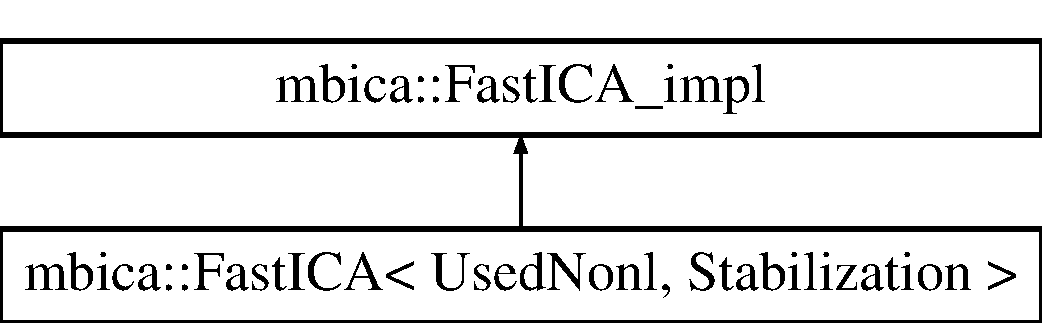
\includegraphics[height=2.000000cm]{classmbica_1_1_fast_i_c_a}
\end{center}
\end{figure}
\subsection*{Public Member Functions}
\begin{DoxyCompactItemize}
\item 
\hyperlink{classmbica_1_1_fast_i_c_a_a0ebfbda8cc36464cd851ae41c29e2ece}{BOOST\_\-PARAMETER\_\-CONSTRUCTOR} (\hyperlink{classmbica_1_1_fast_i_c_a}{FastICA},(\hyperlink{classmbica_1_1_fast_i_c_a__impl}{FastICA\_\-impl}), mbica::tag,(optional(maxIterations,$\ast$)(epsilon,$\ast$)(guessMatrix,$\ast$)(dWh,$\ast$)(wh,$\ast$))) \hyperlink{classmbica_1_1_i_c_a_separator}{ICASeparator} operator()(arma
\end{DoxyCompactItemize}


\subsection{Detailed Description}
\subsubsection*{template$<$class UsedNonl = nonlinearities::Pow$<$3$>$, class Stabilization = NoStabilization$>$ class mbica::FastICA$<$ UsedNonl, Stabilization $>$}

Template class implementing \hyperlink{classmbica_1_1_fast_i_c_a}{FastICA} algorithm for independent component analysis (ICA).


\begin{DoxyParams}{Parameters}
{\em UsedNonl} & Nonlinear function to use when calculating. \\
\hline
{\em Stabilization} & Whether to use stabilized algorithm. \\
\hline
\end{DoxyParams}


Definition at line 143 of file mbica.h.



\subsection{Member Function Documentation}
\hypertarget{classmbica_1_1_fast_i_c_a_a0ebfbda8cc36464cd851ae41c29e2ece}{
\index{mbica::FastICA@{mbica::FastICA}!BOOST\_\-PARAMETER\_\-CONSTRUCTOR@{BOOST\_\-PARAMETER\_\-CONSTRUCTOR}}
\index{BOOST\_\-PARAMETER\_\-CONSTRUCTOR@{BOOST\_\-PARAMETER\_\-CONSTRUCTOR}!mbica::FastICA@{mbica::FastICA}}
\subsubsection[{BOOST\_\-PARAMETER\_\-CONSTRUCTOR}]{\setlength{\rightskip}{0pt plus 5cm}template$<$class UsedNonl = nonlinearities::Pow$<$3$>$, class Stabilization = NoStabilization$>$ {\bf mbica::FastICA}$<$ UsedNonl, Stabilization $>$::BOOST\_\-PARAMETER\_\-CONSTRUCTOR (
\begin{DoxyParamCaption}
\item[{{\bf FastICA}$<$ UsedNonl, Stabilization $>$}]{, }
\item[{({\bf FastICA\_\-impl})}]{, }
\item[{mbica::tag}]{, }
\item[{(optional(maxIterations,$\ast$)(epsilon,$\ast$)(guessMatrix,$\ast$)(dWh,$\ast$)(wh,$\ast$))}]{}
\end{DoxyParamCaption}
)\hspace{0.3cm}{\ttfamily  \mbox{[}inline\mbox{]}}}}
\label{classmbica_1_1_fast_i_c_a_a0ebfbda8cc36464cd851ae41c29e2ece}
Constructor generated by Boost\_\-Parameter libray.

It provides named parameter to ease usage of alogrithm. Parameters can be ommited or given in different order than declared.


\begin{DoxyParams}{Parameters}
{\em \_\-maxIterations} & Maximal number of iterations. If not provided \hyperlink{namespacembica_1_1def_ab5cf75974e06b7a429e0abefa5e2d3c8}{mbica::def::MAX\_\-ITERATIONS} will be set. \\
\hline
{\em \_\-epsilon} & Parameter that says how fast iterations will converge. If not provided \hyperlink{namespacembica_1_1def_a7616a07084967bcb2533a310e68de6b5}{mbica::def::EPSILON} will be set. \\
\hline
{\em \_\-guessMatrix} & Initial matrix that can be given to speed up the calculations. If not provided it will be set to random, orthonormal matrix. \\
\hline
{\em \_\-dWh} & Dewhitening matrix. If not provided it will be calculated. \\
\hline
{\em \_\-wh} & \hyperlink{classmbica_1_1_whitening}{Whitening} matrix. If not provided it will be calculated. Function that actually calculate \hyperlink{classmbica_1_1_fast_i_c_a}{FastICA}.\\
\hline
{\em X} & Matrix with data from which independent components will be calculated. \\
\hline
{\em nIC} & Number of independent components to be found. If set to -\/1 it will take number of dimensions from data matrix. \\
\hline
{\em mu} & Parameter mu. If not provided it's set to \hyperlink{namespacembica_1_1def_a060dcd264ce55c7a950c066dcf7d0a34}{mbica::def::MU}. \\
\hline
\end{DoxyParams}


Definition at line 158 of file mbica.h.



The documentation for this class was generated from the following file:\begin{DoxyCompactItemize}
\item 
include/\hyperlink{mbica_8h}{mbica.h}\end{DoxyCompactItemize}

\hypertarget{classmbica_1_1_fast_i_c_a__impl}{
\section{mbica::FastICA\_\-impl Class Reference}
\label{classmbica_1_1_fast_i_c_a__impl}\index{mbica::FastICA\_\-impl@{mbica::FastICA\_\-impl}}
}


{\ttfamily \#include $<$mbica.h$>$}

Inheritance diagram for mbica::FastICA\_\-impl:\begin{figure}[H]
\begin{center}
\leavevmode
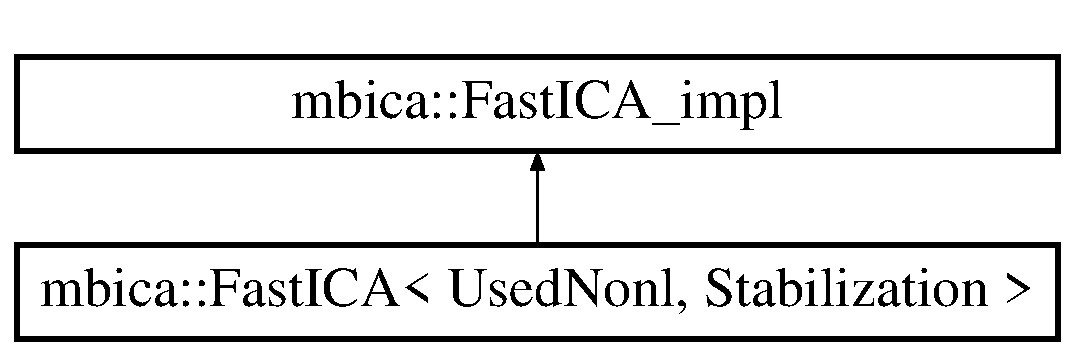
\includegraphics[height=2.000000cm]{classmbica_1_1_fast_i_c_a__impl}
\end{center}
\end{figure}
\subsection*{Public Member Functions}
\begin{DoxyCompactItemize}
\item 
void \hyperlink{classmbica_1_1_fast_i_c_a__impl_acb8a677bfc9539222d05eab68107277c}{setWhiteningMatrix} (arma::mat Wh, arma::mat dWh)
\item 
void \hyperlink{classmbica_1_1_fast_i_c_a__impl_a7bf245e4d88340d45b3ad1319e00724e}{resetWhiteningMatrix} ()
\begin{DoxyCompactList}\small\item\em Method to reset whitening and dewhitening matrixes. \item\end{DoxyCompactList}\item 
const arma::mat \& \hyperlink{classmbica_1_1_fast_i_c_a__impl_a62157ddfa4b2a1fc86a4e490be53a949}{whiteningMatrix} () const 
\begin{DoxyCompactList}\small\item\em Getter of whitening matrix. \item\end{DoxyCompactList}\item 
const arma::mat \& \hyperlink{classmbica_1_1_fast_i_c_a__impl_a820ef876ee9adf2c59102109e8eab248}{dewhiteningMatrix} () const 
\begin{DoxyCompactList}\small\item\em Getter of dewhitening matrix. \item\end{DoxyCompactList}\item 
void \hyperlink{classmbica_1_1_fast_i_c_a__impl_a5dede124e00318eda54452811e1c7ab1}{setEpsilon} (double epsilon)
\item 
double \hyperlink{classmbica_1_1_fast_i_c_a__impl_a7e8502efec4f08a8eb2be77bca7e0c91}{epsilon} () const 
\begin{DoxyCompactList}\small\item\em Getter of epsilon value. \item\end{DoxyCompactList}\item 
void \hyperlink{classmbica_1_1_fast_i_c_a__impl_a1468646012fcdc60f70e3c632a1b9450}{setMaxIterations} (int max)
\begin{DoxyCompactList}\small\item\em Setter of maximal number of iterations. \item\end{DoxyCompactList}\item 
int \hyperlink{classmbica_1_1_fast_i_c_a__impl_a47416533583d0e17176b6ef82316658a}{maxIterations} () const 
\begin{DoxyCompactList}\small\item\em Getter of maximal number of iterations. \item\end{DoxyCompactList}\end{DoxyCompactItemize}
\subsection*{Protected Member Functions}
\begin{DoxyCompactItemize}
\item 
{\footnotesize template$<$class ArgumentPack $>$ }\\\hyperlink{classmbica_1_1_fast_i_c_a__impl_ade2c64db507233e92c06be6f178a1287}{FastICA\_\-impl} (ArgumentPack const \&args)
\end{DoxyCompactItemize}
\subsection*{Protected Attributes}
\begin{DoxyCompactItemize}
\item 
arma::mat \hyperlink{classmbica_1_1_fast_i_c_a__impl_ab1733850788ffd4118563e443cbd12bf}{dWh\_\-}
\item 
arma::mat \hyperlink{classmbica_1_1_fast_i_c_a__impl_a11bb92ab13c2a5d86ee57368a0c6f37b}{Wh\_\-}
\item 
arma::mat \hyperlink{classmbica_1_1_fast_i_c_a__impl_a44e32ead6a78e76dadddd503732bed29}{guess\_\-}
\item 
double \hyperlink{classmbica_1_1_fast_i_c_a__impl_a286ddf4b806607c6b1ff2c01638b562f}{epsilon\_\-}
\item 
int \hyperlink{classmbica_1_1_fast_i_c_a__impl_a33dc4e8644810412d57896fbcd9aed91}{maxIterations\_\-}
\end{DoxyCompactItemize}


\subsection{Detailed Description}
Base class for \hyperlink{classmbica_1_1_fast_i_c_a}{FastICA}.

\begin{DoxyNote}{Note}
It can be only created by \hyperlink{classmbica_1_1_fast_i_c_a}{FastICA} and other derivered classes. 
\end{DoxyNote}


Definition at line 51 of file mbica.h.



\subsection{Constructor \& Destructor Documentation}
\hypertarget{classmbica_1_1_fast_i_c_a__impl_ade2c64db507233e92c06be6f178a1287}{
\index{mbica::FastICA\_\-impl@{mbica::FastICA\_\-impl}!FastICA\_\-impl@{FastICA\_\-impl}}
\index{FastICA\_\-impl@{FastICA\_\-impl}!mbica::FastICA_impl@{mbica::FastICA\_\-impl}}
\subsubsection[{FastICA\_\-impl}]{\setlength{\rightskip}{0pt plus 5cm}template$<$class ArgumentPack $>$ mbica::FastICA\_\-impl::FastICA\_\-impl (
\begin{DoxyParamCaption}
\item[{ArgumentPack const \&}]{args}
\end{DoxyParamCaption}
)\hspace{0.3cm}{\ttfamily  \mbox{[}inline, protected\mbox{]}}}}
\label{classmbica_1_1_fast_i_c_a__impl_ade2c64db507233e92c06be6f178a1287}
Constructor

Special constructor required by Boost\_\-Parameter to provide named parameters in \hyperlink{classmbica_1_1_fast_i_c_a}{FastICA} class.

args Argument provided by Boost\_\-Parameter 

Definition at line 63 of file mbica.h.



\subsection{Member Function Documentation}
\hypertarget{classmbica_1_1_fast_i_c_a__impl_a820ef876ee9adf2c59102109e8eab248}{
\index{mbica::FastICA\_\-impl@{mbica::FastICA\_\-impl}!dewhiteningMatrix@{dewhiteningMatrix}}
\index{dewhiteningMatrix@{dewhiteningMatrix}!mbica::FastICA_impl@{mbica::FastICA\_\-impl}}
\subsubsection[{dewhiteningMatrix}]{\setlength{\rightskip}{0pt plus 5cm}const arma::mat\& mbica::FastICA\_\-impl::dewhiteningMatrix (
\begin{DoxyParamCaption}
{}
\end{DoxyParamCaption}
) const\hspace{0.3cm}{\ttfamily  \mbox{[}inline\mbox{]}}}}
\label{classmbica_1_1_fast_i_c_a__impl_a820ef876ee9adf2c59102109e8eab248}


Getter of dewhitening matrix. 



Definition at line 96 of file mbica.h.

\hypertarget{classmbica_1_1_fast_i_c_a__impl_a7e8502efec4f08a8eb2be77bca7e0c91}{
\index{mbica::FastICA\_\-impl@{mbica::FastICA\_\-impl}!epsilon@{epsilon}}
\index{epsilon@{epsilon}!mbica::FastICA_impl@{mbica::FastICA\_\-impl}}
\subsubsection[{epsilon}]{\setlength{\rightskip}{0pt plus 5cm}double mbica::FastICA\_\-impl::epsilon (
\begin{DoxyParamCaption}
{}
\end{DoxyParamCaption}
) const\hspace{0.3cm}{\ttfamily  \mbox{[}inline\mbox{]}}}}
\label{classmbica_1_1_fast_i_c_a__impl_a7e8502efec4f08a8eb2be77bca7e0c91}


Getter of epsilon value. 



Definition at line 113 of file mbica.h.

\hypertarget{classmbica_1_1_fast_i_c_a__impl_a47416533583d0e17176b6ef82316658a}{
\index{mbica::FastICA\_\-impl@{mbica::FastICA\_\-impl}!maxIterations@{maxIterations}}
\index{maxIterations@{maxIterations}!mbica::FastICA_impl@{mbica::FastICA\_\-impl}}
\subsubsection[{maxIterations}]{\setlength{\rightskip}{0pt plus 5cm}int mbica::FastICA\_\-impl::maxIterations (
\begin{DoxyParamCaption}
{}
\end{DoxyParamCaption}
) const\hspace{0.3cm}{\ttfamily  \mbox{[}inline\mbox{]}}}}
\label{classmbica_1_1_fast_i_c_a__impl_a47416533583d0e17176b6ef82316658a}


Getter of maximal number of iterations. 



Definition at line 123 of file mbica.h.

\hypertarget{classmbica_1_1_fast_i_c_a__impl_a7bf245e4d88340d45b3ad1319e00724e}{
\index{mbica::FastICA\_\-impl@{mbica::FastICA\_\-impl}!resetWhiteningMatrix@{resetWhiteningMatrix}}
\index{resetWhiteningMatrix@{resetWhiteningMatrix}!mbica::FastICA_impl@{mbica::FastICA\_\-impl}}
\subsubsection[{resetWhiteningMatrix}]{\setlength{\rightskip}{0pt plus 5cm}void mbica::FastICA\_\-impl::resetWhiteningMatrix (
\begin{DoxyParamCaption}
{}
\end{DoxyParamCaption}
)\hspace{0.3cm}{\ttfamily  \mbox{[}inline\mbox{]}}}}
\label{classmbica_1_1_fast_i_c_a__impl_a7bf245e4d88340d45b3ad1319e00724e}


Method to reset whitening and dewhitening matrixes. 



Definition at line 85 of file mbica.h.

\hypertarget{classmbica_1_1_fast_i_c_a__impl_a5dede124e00318eda54452811e1c7ab1}{
\index{mbica::FastICA\_\-impl@{mbica::FastICA\_\-impl}!setEpsilon@{setEpsilon}}
\index{setEpsilon@{setEpsilon}!mbica::FastICA_impl@{mbica::FastICA\_\-impl}}
\subsubsection[{setEpsilon}]{\setlength{\rightskip}{0pt plus 5cm}void mbica::FastICA\_\-impl::setEpsilon (
\begin{DoxyParamCaption}
\item[{double}]{epsilon}
\end{DoxyParamCaption}
)\hspace{0.3cm}{\ttfamily  \mbox{[}inline\mbox{]}}}}
\label{classmbica_1_1_fast_i_c_a__impl_a5dede124e00318eda54452811e1c7ab1}
Setter of epsilon.

Epsilon is a parameter that says how fast iterations will converge. The smaller epsilon is the harder to converge.


\begin{DoxyParams}{Parameters}
{\em epsilon} & New value of epsilon. \\
\hline
\end{DoxyParams}


Definition at line 108 of file mbica.h.

\hypertarget{classmbica_1_1_fast_i_c_a__impl_a1468646012fcdc60f70e3c632a1b9450}{
\index{mbica::FastICA\_\-impl@{mbica::FastICA\_\-impl}!setMaxIterations@{setMaxIterations}}
\index{setMaxIterations@{setMaxIterations}!mbica::FastICA_impl@{mbica::FastICA\_\-impl}}
\subsubsection[{setMaxIterations}]{\setlength{\rightskip}{0pt plus 5cm}void mbica::FastICA\_\-impl::setMaxIterations (
\begin{DoxyParamCaption}
\item[{int}]{max}
\end{DoxyParamCaption}
)\hspace{0.3cm}{\ttfamily  \mbox{[}inline\mbox{]}}}}
\label{classmbica_1_1_fast_i_c_a__impl_a1468646012fcdc60f70e3c632a1b9450}


Setter of maximal number of iterations. 



Definition at line 118 of file mbica.h.

\hypertarget{classmbica_1_1_fast_i_c_a__impl_acb8a677bfc9539222d05eab68107277c}{
\index{mbica::FastICA\_\-impl@{mbica::FastICA\_\-impl}!setWhiteningMatrix@{setWhiteningMatrix}}
\index{setWhiteningMatrix@{setWhiteningMatrix}!mbica::FastICA_impl@{mbica::FastICA\_\-impl}}
\subsubsection[{setWhiteningMatrix}]{\setlength{\rightskip}{0pt plus 5cm}void mbica::FastICA\_\-impl::setWhiteningMatrix (
\begin{DoxyParamCaption}
\item[{arma::mat}]{Wh, }
\item[{arma::mat}]{dWh}
\end{DoxyParamCaption}
)\hspace{0.3cm}{\ttfamily  \mbox{[}inline\mbox{]}}}}
\label{classmbica_1_1_fast_i_c_a__impl_acb8a677bfc9539222d05eab68107277c}
Setter of whitening/dewhitening matrixes.


\begin{DoxyParams}{Parameters}
{\em Wh} & \hyperlink{classmbica_1_1_whitening}{Whitening} matrix. \\
\hline
{\em dWh} & Dewhitening matrix. \\
\hline
\end{DoxyParams}


Definition at line 79 of file mbica.h.

\hypertarget{classmbica_1_1_fast_i_c_a__impl_a62157ddfa4b2a1fc86a4e490be53a949}{
\index{mbica::FastICA\_\-impl@{mbica::FastICA\_\-impl}!whiteningMatrix@{whiteningMatrix}}
\index{whiteningMatrix@{whiteningMatrix}!mbica::FastICA_impl@{mbica::FastICA\_\-impl}}
\subsubsection[{whiteningMatrix}]{\setlength{\rightskip}{0pt plus 5cm}const arma::mat\& mbica::FastICA\_\-impl::whiteningMatrix (
\begin{DoxyParamCaption}
{}
\end{DoxyParamCaption}
) const\hspace{0.3cm}{\ttfamily  \mbox{[}inline\mbox{]}}}}
\label{classmbica_1_1_fast_i_c_a__impl_a62157ddfa4b2a1fc86a4e490be53a949}


Getter of whitening matrix. 



Definition at line 91 of file mbica.h.



\subsection{Member Data Documentation}
\hypertarget{classmbica_1_1_fast_i_c_a__impl_ab1733850788ffd4118563e443cbd12bf}{
\index{mbica::FastICA\_\-impl@{mbica::FastICA\_\-impl}!dWh\_\-@{dWh\_\-}}
\index{dWh\_\-@{dWh\_\-}!mbica::FastICA_impl@{mbica::FastICA\_\-impl}}
\subsubsection[{dWh\_\-}]{\setlength{\rightskip}{0pt plus 5cm}arma::mat {\bf mbica::FastICA\_\-impl::dWh\_\-}\hspace{0.3cm}{\ttfamily  \mbox{[}protected\mbox{]}}}}
\label{classmbica_1_1_fast_i_c_a__impl_ab1733850788ffd4118563e443cbd12bf}


Definition at line 128 of file mbica.h.

\hypertarget{classmbica_1_1_fast_i_c_a__impl_a286ddf4b806607c6b1ff2c01638b562f}{
\index{mbica::FastICA\_\-impl@{mbica::FastICA\_\-impl}!epsilon\_\-@{epsilon\_\-}}
\index{epsilon\_\-@{epsilon\_\-}!mbica::FastICA_impl@{mbica::FastICA\_\-impl}}
\subsubsection[{epsilon\_\-}]{\setlength{\rightskip}{0pt plus 5cm}double {\bf mbica::FastICA\_\-impl::epsilon\_\-}\hspace{0.3cm}{\ttfamily  \mbox{[}protected\mbox{]}}}}
\label{classmbica_1_1_fast_i_c_a__impl_a286ddf4b806607c6b1ff2c01638b562f}


Definition at line 131 of file mbica.h.

\hypertarget{classmbica_1_1_fast_i_c_a__impl_a44e32ead6a78e76dadddd503732bed29}{
\index{mbica::FastICA\_\-impl@{mbica::FastICA\_\-impl}!guess\_\-@{guess\_\-}}
\index{guess\_\-@{guess\_\-}!mbica::FastICA_impl@{mbica::FastICA\_\-impl}}
\subsubsection[{guess\_\-}]{\setlength{\rightskip}{0pt plus 5cm}arma::mat {\bf mbica::FastICA\_\-impl::guess\_\-}\hspace{0.3cm}{\ttfamily  \mbox{[}protected\mbox{]}}}}
\label{classmbica_1_1_fast_i_c_a__impl_a44e32ead6a78e76dadddd503732bed29}


Definition at line 130 of file mbica.h.

\hypertarget{classmbica_1_1_fast_i_c_a__impl_a33dc4e8644810412d57896fbcd9aed91}{
\index{mbica::FastICA\_\-impl@{mbica::FastICA\_\-impl}!maxIterations\_\-@{maxIterations\_\-}}
\index{maxIterations\_\-@{maxIterations\_\-}!mbica::FastICA_impl@{mbica::FastICA\_\-impl}}
\subsubsection[{maxIterations\_\-}]{\setlength{\rightskip}{0pt plus 5cm}int {\bf mbica::FastICA\_\-impl::maxIterations\_\-}\hspace{0.3cm}{\ttfamily  \mbox{[}protected\mbox{]}}}}
\label{classmbica_1_1_fast_i_c_a__impl_a33dc4e8644810412d57896fbcd9aed91}


Definition at line 132 of file mbica.h.

\hypertarget{classmbica_1_1_fast_i_c_a__impl_a11bb92ab13c2a5d86ee57368a0c6f37b}{
\index{mbica::FastICA\_\-impl@{mbica::FastICA\_\-impl}!Wh\_\-@{Wh\_\-}}
\index{Wh\_\-@{Wh\_\-}!mbica::FastICA_impl@{mbica::FastICA\_\-impl}}
\subsubsection[{Wh\_\-}]{\setlength{\rightskip}{0pt plus 5cm}arma::mat {\bf mbica::FastICA\_\-impl::Wh\_\-}\hspace{0.3cm}{\ttfamily  \mbox{[}protected\mbox{]}}}}
\label{classmbica_1_1_fast_i_c_a__impl_a11bb92ab13c2a5d86ee57368a0c6f37b}


Definition at line 129 of file mbica.h.



The documentation for this class was generated from the following file:\begin{DoxyCompactItemize}
\item 
include/\hyperlink{mbica_8h}{mbica.h}\end{DoxyCompactItemize}

\hypertarget{classmbica_1_1nonlinearities_1_1_gauss}{
\section{mbica::nonlinearities::Gauss$<$ a, b $>$ Class Template Reference}
\label{classmbica_1_1nonlinearities_1_1_gauss}\index{mbica::nonlinearities::Gauss@{mbica::nonlinearities::Gauss}}
}


{\ttfamily \#include $<$nonlinearities.h$>$}

Inheritance diagram for mbica::nonlinearities::Gauss$<$ a, b $>$:\begin{figure}[H]
\begin{center}
\leavevmode
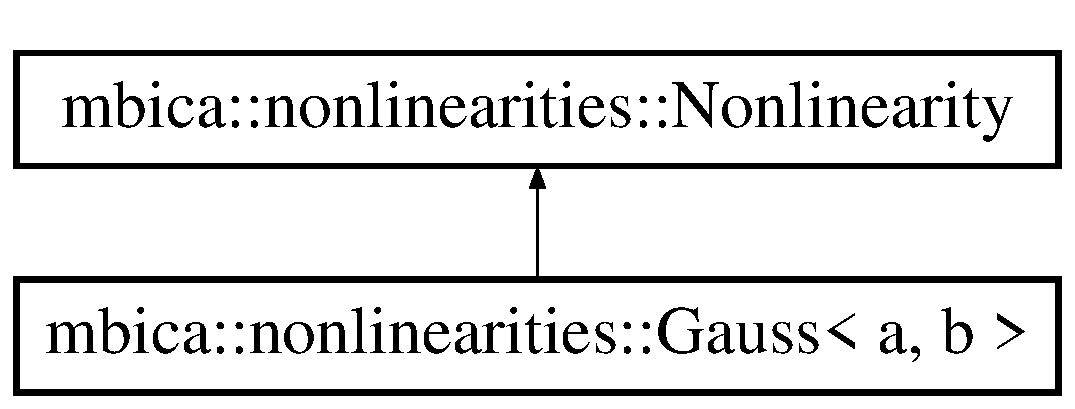
\includegraphics[height=2.000000cm]{classmbica_1_1nonlinearities_1_1_gauss}
\end{center}
\end{figure}
\subsection*{Public Member Functions}
\begin{DoxyCompactItemize}
\item 
\hyperlink{classmbica_1_1nonlinearities_1_1_gauss_a14780d268824e70e1b33988120092b81}{Gauss} (arma::mat X)
\end{DoxyCompactItemize}


\subsection{Detailed Description}
\subsubsection*{template$<$int a = 1, int b = 1$>$ class mbica::nonlinearities::Gauss$<$ a, b $>$}

Class implementing gauss nonlinearity.

\begin{DoxyNote}{Note}
Class uses fraction a/b as a parameter.
\end{DoxyNote}

\begin{DoxyParams}{Parameters}
{\em a} & Numerator of parameter. \\
\hline
{\em b} & Denominator of parameter. \\
\hline
\end{DoxyParams}


Definition at line 83 of file nonlinearities.h.



\subsection{Constructor \& Destructor Documentation}
\hypertarget{classmbica_1_1nonlinearities_1_1_gauss_a14780d268824e70e1b33988120092b81}{
\index{mbica::nonlinearities::Gauss@{mbica::nonlinearities::Gauss}!Gauss@{Gauss}}
\index{Gauss@{Gauss}!mbica::nonlinearities::Gauss@{mbica::nonlinearities::Gauss}}
\subsubsection[{Gauss}]{\setlength{\rightskip}{0pt plus 5cm}template$<$int a = 1, int b = 1$>$ {\bf mbica::nonlinearities::Gauss}$<$ a, b $>$::{\bf Gauss} (
\begin{DoxyParamCaption}
\item[{arma::mat}]{X}
\end{DoxyParamCaption}
)\hspace{0.3cm}{\ttfamily  \mbox{[}inline\mbox{]}}}}
\label{classmbica_1_1nonlinearities_1_1_gauss_a14780d268824e70e1b33988120092b81}


Definition at line 85 of file nonlinearities.h.



The documentation for this class was generated from the following file:\begin{DoxyCompactItemize}
\item 
include/\hyperlink{nonlinearities_8h}{nonlinearities.h}\end{DoxyCompactItemize}

\hypertarget{classmbica_1_1_i_c_a_separator}{
\section{mbica::ICASeparator Class Reference}
\label{classmbica_1_1_i_c_a_separator}\index{mbica::ICASeparator@{mbica::ICASeparator}}
}


{\ttfamily \#include $<$icaseparator.h$>$}

\subsection*{Public Member Functions}
\begin{DoxyCompactItemize}
\item 
\hyperlink{classmbica_1_1_i_c_a_separator_ab1d0874ff943f2b3c04888768c032eb1}{ICASeparator} (arma::mat A, arma::mat W)
\item 
arma::mat \hyperlink{classmbica_1_1_i_c_a_separator_a1aa13483c85507e86ac9fe4465e709f7}{operator()} (arma::mat X)
\item 
arma::mat \hyperlink{classmbica_1_1_i_c_a_separator_aa6e102581e99e56bee0b21cf6be8fbe0}{mixSignals} (arma::mat S)
\item 
const arma::mat \& \hyperlink{classmbica_1_1_i_c_a_separator_a2ae50bb7ba10c9e177dc8d3d7e54dfdf}{getA} () const 
\begin{DoxyCompactList}\small\item\em Getter of mixing matrix. \item\end{DoxyCompactList}\item 
const arma::mat \& \hyperlink{classmbica_1_1_i_c_a_separator_ac9cc05d9ca89d9bdab7ba0dc9b9e3a69}{getW} () const 
\begin{DoxyCompactList}\small\item\em Getter of unmixing matrix. \item\end{DoxyCompactList}\end{DoxyCompactItemize}


\subsection{Detailed Description}
Class that provides easy way to count independent components. 

Definition at line 20 of file icaseparator.h.



\subsection{Constructor \& Destructor Documentation}
\hypertarget{classmbica_1_1_i_c_a_separator_ab1d0874ff943f2b3c04888768c032eb1}{
\index{mbica::ICASeparator@{mbica::ICASeparator}!ICASeparator@{ICASeparator}}
\index{ICASeparator@{ICASeparator}!mbica::ICASeparator@{mbica::ICASeparator}}
\subsubsection[{ICASeparator}]{\setlength{\rightskip}{0pt plus 5cm}mbica::ICASeparator::ICASeparator (
\begin{DoxyParamCaption}
\item[{arma::mat}]{A, }
\item[{arma::mat}]{W}
\end{DoxyParamCaption}
)\hspace{0.3cm}{\ttfamily  \mbox{[}inline\mbox{]}}}}
\label{classmbica_1_1_i_c_a_separator_ab1d0874ff943f2b3c04888768c032eb1}
Constructor.


\begin{DoxyParams}{Parameters}
{\em A} & Mixing matrix. \\
\hline
{\em W} & Unmixing matrix. \\
\hline
\end{DoxyParams}


Definition at line 29 of file icaseparator.h.



\subsection{Member Function Documentation}
\hypertarget{classmbica_1_1_i_c_a_separator_a2ae50bb7ba10c9e177dc8d3d7e54dfdf}{
\index{mbica::ICASeparator@{mbica::ICASeparator}!getA@{getA}}
\index{getA@{getA}!mbica::ICASeparator@{mbica::ICASeparator}}
\subsubsection[{getA}]{\setlength{\rightskip}{0pt plus 5cm}const arma::mat\& mbica::ICASeparator::getA (
\begin{DoxyParamCaption}
{}
\end{DoxyParamCaption}
) const\hspace{0.3cm}{\ttfamily  \mbox{[}inline\mbox{]}}}}
\label{classmbica_1_1_i_c_a_separator_a2ae50bb7ba10c9e177dc8d3d7e54dfdf}


Getter of mixing matrix. 



Definition at line 56 of file icaseparator.h.

\hypertarget{classmbica_1_1_i_c_a_separator_ac9cc05d9ca89d9bdab7ba0dc9b9e3a69}{
\index{mbica::ICASeparator@{mbica::ICASeparator}!getW@{getW}}
\index{getW@{getW}!mbica::ICASeparator@{mbica::ICASeparator}}
\subsubsection[{getW}]{\setlength{\rightskip}{0pt plus 5cm}const arma::mat\& mbica::ICASeparator::getW (
\begin{DoxyParamCaption}
{}
\end{DoxyParamCaption}
) const\hspace{0.3cm}{\ttfamily  \mbox{[}inline\mbox{]}}}}
\label{classmbica_1_1_i_c_a_separator_ac9cc05d9ca89d9bdab7ba0dc9b9e3a69}


Getter of unmixing matrix. 



Definition at line 61 of file icaseparator.h.

\hypertarget{classmbica_1_1_i_c_a_separator_aa6e102581e99e56bee0b21cf6be8fbe0}{
\index{mbica::ICASeparator@{mbica::ICASeparator}!mixSignals@{mixSignals}}
\index{mixSignals@{mixSignals}!mbica::ICASeparator@{mbica::ICASeparator}}
\subsubsection[{mixSignals}]{\setlength{\rightskip}{0pt plus 5cm}arma::mat mbica::ICASeparator::mixSignals (
\begin{DoxyParamCaption}
\item[{arma::mat}]{S}
\end{DoxyParamCaption}
)\hspace{0.3cm}{\ttfamily  \mbox{[}inline\mbox{]}}}}
\label{classmbica_1_1_i_c_a_separator_aa6e102581e99e56bee0b21cf6be8fbe0}
Method that mixes given signals


\begin{DoxyParams}{Parameters}
{\em S} & Matrix to be mixed. \\
\hline
\end{DoxyParams}
\begin{DoxyReturn}{Returns}
Matrix with mixed data. 
\end{DoxyReturn}


Definition at line 51 of file icaseparator.h.

\hypertarget{classmbica_1_1_i_c_a_separator_a1aa13483c85507e86ac9fe4465e709f7}{
\index{mbica::ICASeparator@{mbica::ICASeparator}!operator()@{operator()}}
\index{operator()@{operator()}!mbica::ICASeparator@{mbica::ICASeparator}}
\subsubsection[{operator()}]{\setlength{\rightskip}{0pt plus 5cm}arma::mat mbica::ICASeparator::operator() (
\begin{DoxyParamCaption}
\item[{arma::mat}]{X}
\end{DoxyParamCaption}
)\hspace{0.3cm}{\ttfamily  \mbox{[}inline\mbox{]}}}}
\label{classmbica_1_1_i_c_a_separator_a1aa13483c85507e86ac9fe4465e709f7}
Method that unmix given signal.


\begin{DoxyParams}{Parameters}
{\em X} & Matrix with mixed signal. \\
\hline
\end{DoxyParams}
\begin{DoxyReturn}{Returns}
Matrix with unmixed signal. 
\end{DoxyReturn}


Definition at line 41 of file icaseparator.h.



The documentation for this class was generated from the following file:\begin{DoxyCompactItemize}
\item 
include/\hyperlink{icaseparator_8h}{icaseparator.h}\end{DoxyCompactItemize}

\hypertarget{classmbica_1_1nonlinearities_1_1_nonlinearity}{
\section{mbica::nonlinearities::Nonlinearity Class Reference}
\label{classmbica_1_1nonlinearities_1_1_nonlinearity}\index{mbica::nonlinearities::Nonlinearity@{mbica::nonlinearities::Nonlinearity}}
}


{\ttfamily \#include $<$nonlinearities.h$>$}

Inheritance diagram for mbica::nonlinearities::Nonlinearity:\begin{figure}[H]
\begin{center}
\leavevmode
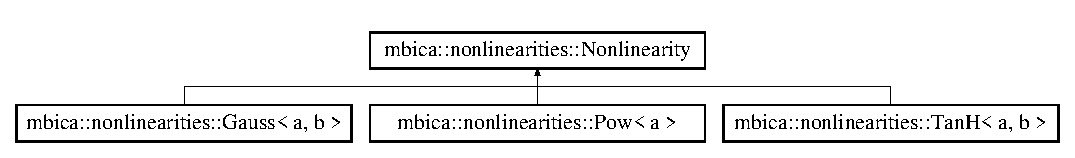
\includegraphics[height=1.681682cm]{classmbica_1_1nonlinearities_1_1_nonlinearity}
\end{center}
\end{figure}
\subsection*{Public Member Functions}
\begin{DoxyCompactItemize}
\item 
arma::mat \hyperlink{classmbica_1_1nonlinearities_1_1_nonlinearity_a2fdac4cb3e02508f70b79af06a9a6487}{G} ()
\begin{DoxyCompactList}\small\item\em Method returning value of function. \item\end{DoxyCompactList}\item 
arma::mat \hyperlink{classmbica_1_1nonlinearities_1_1_nonlinearity_a49e21ebf1f1f0d9e400b864cd75cec76}{dG} ()
\begin{DoxyCompactList}\small\item\em Method returning value of derivative of function. \item\end{DoxyCompactList}\end{DoxyCompactItemize}
\subsection*{Protected Member Functions}
\begin{DoxyCompactItemize}
\item 
\hyperlink{classmbica_1_1nonlinearities_1_1_nonlinearity_ab5cffa8d6f796bf97b2135f35c0b0d9a}{Nonlinearity} ()
\begin{DoxyCompactList}\small\item\em Protected constructor to prevent from creating \hyperlink{classmbica_1_1nonlinearities_1_1_nonlinearity}{Nonlinearity} objects. \item\end{DoxyCompactList}\end{DoxyCompactItemize}
\subsection*{Protected Attributes}
\begin{DoxyCompactItemize}
\item 
arma::mat \hyperlink{classmbica_1_1nonlinearities_1_1_nonlinearity_a11ae531b284349515331e05021a33ea9}{g\_\-}
\item 
arma::mat \hyperlink{classmbica_1_1nonlinearities_1_1_nonlinearity_a7e88146ea0876175cd9834af14aee58a}{dg\_\-}
\end{DoxyCompactItemize}


\subsection{Detailed Description}
Base class for preimplemented nonlinearities. 

Definition at line 25 of file nonlinearities.h.



\subsection{Constructor \& Destructor Documentation}
\hypertarget{classmbica_1_1nonlinearities_1_1_nonlinearity_ab5cffa8d6f796bf97b2135f35c0b0d9a}{
\index{mbica::nonlinearities::Nonlinearity@{mbica::nonlinearities::Nonlinearity}!Nonlinearity@{Nonlinearity}}
\index{Nonlinearity@{Nonlinearity}!mbica::nonlinearities::Nonlinearity@{mbica::nonlinearities::Nonlinearity}}
\subsubsection[{Nonlinearity}]{\setlength{\rightskip}{0pt plus 5cm}mbica::nonlinearities::Nonlinearity::Nonlinearity (
\begin{DoxyParamCaption}
{}
\end{DoxyParamCaption}
)\hspace{0.3cm}{\ttfamily  \mbox{[}inline, protected\mbox{]}}}}
\label{classmbica_1_1nonlinearities_1_1_nonlinearity_ab5cffa8d6f796bf97b2135f35c0b0d9a}


Protected constructor to prevent from creating \hyperlink{classmbica_1_1nonlinearities_1_1_nonlinearity}{Nonlinearity} objects. 



Definition at line 34 of file nonlinearities.h.



\subsection{Member Function Documentation}
\hypertarget{classmbica_1_1nonlinearities_1_1_nonlinearity_a49e21ebf1f1f0d9e400b864cd75cec76}{
\index{mbica::nonlinearities::Nonlinearity@{mbica::nonlinearities::Nonlinearity}!dG@{dG}}
\index{dG@{dG}!mbica::nonlinearities::Nonlinearity@{mbica::nonlinearities::Nonlinearity}}
\subsubsection[{dG}]{\setlength{\rightskip}{0pt plus 5cm}arma::mat mbica::nonlinearities::Nonlinearity::dG (
\begin{DoxyParamCaption}
{}
\end{DoxyParamCaption}
)\hspace{0.3cm}{\ttfamily  \mbox{[}inline\mbox{]}}}}
\label{classmbica_1_1nonlinearities_1_1_nonlinearity_a49e21ebf1f1f0d9e400b864cd75cec76}


Method returning value of derivative of function. 



Definition at line 30 of file nonlinearities.h.

\hypertarget{classmbica_1_1nonlinearities_1_1_nonlinearity_a2fdac4cb3e02508f70b79af06a9a6487}{
\index{mbica::nonlinearities::Nonlinearity@{mbica::nonlinearities::Nonlinearity}!G@{G}}
\index{G@{G}!mbica::nonlinearities::Nonlinearity@{mbica::nonlinearities::Nonlinearity}}
\subsubsection[{G}]{\setlength{\rightskip}{0pt plus 5cm}arma::mat mbica::nonlinearities::Nonlinearity::G (
\begin{DoxyParamCaption}
{}
\end{DoxyParamCaption}
)\hspace{0.3cm}{\ttfamily  \mbox{[}inline\mbox{]}}}}
\label{classmbica_1_1nonlinearities_1_1_nonlinearity_a2fdac4cb3e02508f70b79af06a9a6487}


Method returning value of function. 



Definition at line 28 of file nonlinearities.h.



\subsection{Member Data Documentation}
\hypertarget{classmbica_1_1nonlinearities_1_1_nonlinearity_a7e88146ea0876175cd9834af14aee58a}{
\index{mbica::nonlinearities::Nonlinearity@{mbica::nonlinearities::Nonlinearity}!dg\_\-@{dg\_\-}}
\index{dg\_\-@{dg\_\-}!mbica::nonlinearities::Nonlinearity@{mbica::nonlinearities::Nonlinearity}}
\subsubsection[{dg\_\-}]{\setlength{\rightskip}{0pt plus 5cm}arma::mat {\bf mbica::nonlinearities::Nonlinearity::dg\_\-}\hspace{0.3cm}{\ttfamily  \mbox{[}protected\mbox{]}}}}
\label{classmbica_1_1nonlinearities_1_1_nonlinearity_a7e88146ea0876175cd9834af14aee58a}


Definition at line 38 of file nonlinearities.h.

\hypertarget{classmbica_1_1nonlinearities_1_1_nonlinearity_a11ae531b284349515331e05021a33ea9}{
\index{mbica::nonlinearities::Nonlinearity@{mbica::nonlinearities::Nonlinearity}!g\_\-@{g\_\-}}
\index{g\_\-@{g\_\-}!mbica::nonlinearities::Nonlinearity@{mbica::nonlinearities::Nonlinearity}}
\subsubsection[{g\_\-}]{\setlength{\rightskip}{0pt plus 5cm}arma::mat {\bf mbica::nonlinearities::Nonlinearity::g\_\-}\hspace{0.3cm}{\ttfamily  \mbox{[}protected\mbox{]}}}}
\label{classmbica_1_1nonlinearities_1_1_nonlinearity_a11ae531b284349515331e05021a33ea9}


Definition at line 37 of file nonlinearities.h.



The documentation for this class was generated from the following file:\begin{DoxyCompactItemize}
\item 
include/\hyperlink{nonlinearities_8h}{nonlinearities.h}\end{DoxyCompactItemize}

\hypertarget{classmbica_1_1_no_stabilization}{
\section{mbica::NoStabilization Class Reference}
\label{classmbica_1_1_no_stabilization}\index{mbica::NoStabilization@{mbica::NoStabilization}}
}


{\ttfamily \#include $<$policies.h$>$}

\subsection*{Public Member Functions}
\begin{DoxyCompactItemize}
\item 
\hyperlink{classmbica_1_1_no_stabilization_a5fbdc1ae0eabc002d7db9199d2b94717}{NoStabilization} (double, double, int)
\item 
void \hyperlink{classmbica_1_1_no_stabilization_a6e356d0bf7e0f6511d29e8ab6feb94e5}{operator()} (int, const arma::mat \&, const arma::mat \&)
\end{DoxyCompactItemize}


\subsection{Detailed Description}
Empty class that doesn't provide stabilization. 

Definition at line 21 of file policies.h.



\subsection{Constructor \& Destructor Documentation}
\hypertarget{classmbica_1_1_no_stabilization_a5fbdc1ae0eabc002d7db9199d2b94717}{
\index{mbica::NoStabilization@{mbica::NoStabilization}!NoStabilization@{NoStabilization}}
\index{NoStabilization@{NoStabilization}!mbica::NoStabilization@{mbica::NoStabilization}}
\subsubsection[{NoStabilization}]{\setlength{\rightskip}{0pt plus 5cm}mbica::NoStabilization::NoStabilization (
\begin{DoxyParamCaption}
\item[{double}]{, }
\item[{double}]{, }
\item[{int}]{}
\end{DoxyParamCaption}
)\hspace{0.3cm}{\ttfamily  \mbox{[}inline\mbox{]}}}}
\label{classmbica_1_1_no_stabilization_a5fbdc1ae0eabc002d7db9199d2b94717}


Definition at line 23 of file policies.h.



\subsection{Member Function Documentation}
\hypertarget{classmbica_1_1_no_stabilization_a6e356d0bf7e0f6511d29e8ab6feb94e5}{
\index{mbica::NoStabilization@{mbica::NoStabilization}!operator()@{operator()}}
\index{operator()@{operator()}!mbica::NoStabilization@{mbica::NoStabilization}}
\subsubsection[{operator()}]{\setlength{\rightskip}{0pt plus 5cm}void mbica::NoStabilization::operator() (
\begin{DoxyParamCaption}
\item[{int}]{, }
\item[{const arma::mat \&}]{, }
\item[{const arma::mat \&}]{}
\end{DoxyParamCaption}
)\hspace{0.3cm}{\ttfamily  \mbox{[}inline\mbox{]}}}}
\label{classmbica_1_1_no_stabilization_a6e356d0bf7e0f6511d29e8ab6feb94e5}


Definition at line 24 of file policies.h.



The documentation for this class was generated from the following file:\begin{DoxyCompactItemize}
\item 
include/\hyperlink{policies_8h}{policies.h}\end{DoxyCompactItemize}

\hypertarget{classmbica_1_1_p_c_a}{
\section{mbica::PCA Class Reference}
\label{classmbica_1_1_p_c_a}\index{mbica::PCA@{mbica::PCA}}
}


{\ttfamily \#include $<$utils.h$>$}

\subsection*{Public Member Functions}
\begin{DoxyCompactItemize}
\item 
void \hyperlink{classmbica_1_1_p_c_a_a8ea74ed9daf02d1fed1ec0ecf478fa8d}{operator()} (const arma::mat \&X, arma::mat \&E, arma::vec \&D)
\end{DoxyCompactItemize}


\subsection{Detailed Description}
Class implementing primary component analisis (\hyperlink{classmbica_1_1_p_c_a}{PCA}). 

Definition at line 30 of file utils.h.



\subsection{Member Function Documentation}
\hypertarget{classmbica_1_1_p_c_a_a8ea74ed9daf02d1fed1ec0ecf478fa8d}{
\index{mbica::PCA@{mbica::PCA}!operator()@{operator()}}
\index{operator()@{operator()}!mbica::PCA@{mbica::PCA}}
\subsubsection[{operator()}]{\setlength{\rightskip}{0pt plus 5cm}void mbica::PCA::operator() (
\begin{DoxyParamCaption}
\item[{const arma::mat \&}]{X, }
\item[{arma::mat \&}]{E, }
\item[{arma::vec \&}]{D}
\end{DoxyParamCaption}
)}}
\label{classmbica_1_1_p_c_a_a8ea74ed9daf02d1fed1ec0ecf478fa8d}
Function that calculaates transformation matrix.


\begin{DoxyParams}{Parameters}
{\em X} & Matrix with data on which \hyperlink{classmbica_1_1_p_c_a}{PCA} will be calculated. Samples should be in columns. \\
\hline
{\em E} & Output parameter which returns matrix with eigenvectorsin rows, which can be used as transofmration matrix. \\
\hline
{\em D} & Output parameter which returns vector with eigenvalues. \\
\hline
\end{DoxyParams}


Definition at line 15 of file utils.cpp.



The documentation for this class was generated from the following files:\begin{DoxyCompactItemize}
\item 
include/\hyperlink{utils_8h}{utils.h}\item 
source/\hyperlink{utils_8cpp}{utils.cpp}\end{DoxyCompactItemize}

\hypertarget{classmbica_1_1nonlinearities_1_1_pow}{
\section{mbica::nonlinearities::Pow$<$ a $>$ Class Template Reference}
\label{classmbica_1_1nonlinearities_1_1_pow}\index{mbica::nonlinearities::Pow@{mbica::nonlinearities::Pow}}
}


{\ttfamily \#include $<$nonlinearities.h$>$}

Inheritance diagram for mbica::nonlinearities::Pow$<$ a $>$:\begin{figure}[H]
\begin{center}
\leavevmode
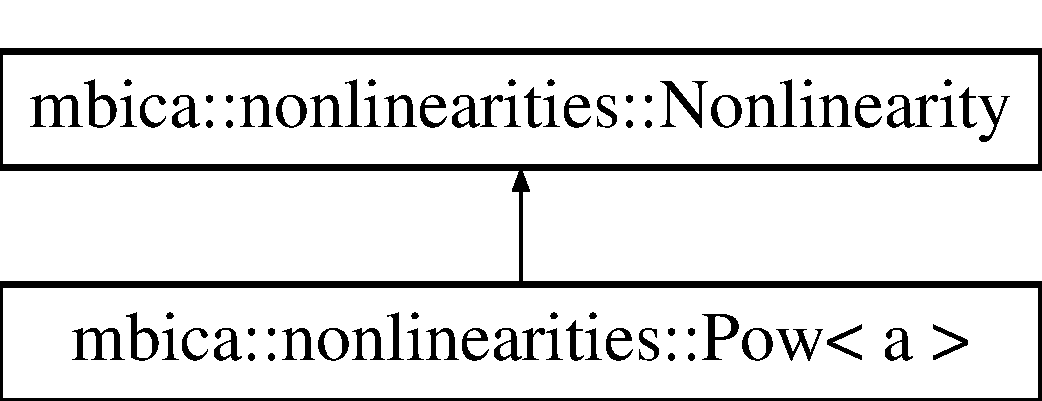
\includegraphics[height=2.000000cm]{classmbica_1_1nonlinearities_1_1_pow}
\end{center}
\end{figure}
\subsection*{Public Member Functions}
\begin{DoxyCompactItemize}
\item 
\hyperlink{classmbica_1_1nonlinearities_1_1_pow_a66f32832f6abd8f88c40351a94824cec}{Pow} (arma::mat X)
\end{DoxyCompactItemize}


\subsection{Detailed Description}
\subsubsection*{template$<$int a = 3$>$ class mbica::nonlinearities::Pow$<$ a $>$}

Class implementing power function on matrix elements.


\begin{DoxyParams}{Parameters}
{\em a} & Exponent. \\
\hline
\end{DoxyParams}


Definition at line 47 of file nonlinearities.h.



\subsection{Constructor \& Destructor Documentation}
\hypertarget{classmbica_1_1nonlinearities_1_1_pow_a66f32832f6abd8f88c40351a94824cec}{
\index{mbica::nonlinearities::Pow@{mbica::nonlinearities::Pow}!Pow@{Pow}}
\index{Pow@{Pow}!mbica::nonlinearities::Pow@{mbica::nonlinearities::Pow}}
\subsubsection[{Pow}]{\setlength{\rightskip}{0pt plus 5cm}template$<$int a = 3$>$ {\bf mbica::nonlinearities::Pow}$<$ a $>$::{\bf Pow} (
\begin{DoxyParamCaption}
\item[{arma::mat}]{X}
\end{DoxyParamCaption}
)\hspace{0.3cm}{\ttfamily  \mbox{[}inline\mbox{]}}}}
\label{classmbica_1_1nonlinearities_1_1_pow_a66f32832f6abd8f88c40351a94824cec}


Definition at line 49 of file nonlinearities.h.



The documentation for this class was generated from the following file:\begin{DoxyCompactItemize}
\item 
include/\hyperlink{nonlinearities_8h}{nonlinearities.h}\end{DoxyCompactItemize}

\hypertarget{classmbica_1_1nonlinearities_1_1_tan_h}{
\section{mbica::nonlinearities::TanH$<$ a, b $>$ Class Template Reference}
\label{classmbica_1_1nonlinearities_1_1_tan_h}\index{mbica::nonlinearities::TanH@{mbica::nonlinearities::TanH}}
}


{\ttfamily \#include $<$nonlinearities.h$>$}

Inheritance diagram for mbica::nonlinearities::TanH$<$ a, b $>$:\begin{figure}[H]
\begin{center}
\leavevmode
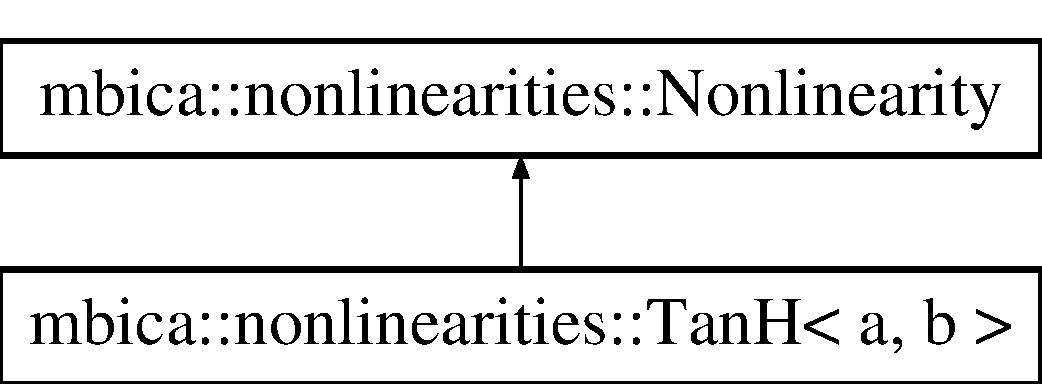
\includegraphics[height=2.000000cm]{classmbica_1_1nonlinearities_1_1_tan_h}
\end{center}
\end{figure}
\subsection*{Public Member Functions}
\begin{DoxyCompactItemize}
\item 
\hyperlink{classmbica_1_1nonlinearities_1_1_tan_h_aa77bdf08978739b666d996c1cb2ab076}{TanH} (arma::mat X)
\end{DoxyCompactItemize}


\subsection{Detailed Description}
\subsubsection*{template$<$int a = 1, int b = 1$>$ class mbica::nonlinearities::TanH$<$ a, b $>$}

Class implementing tanh nonlinearity.

\begin{DoxyNote}{Note}
Class uses fraction a/b as a parameter.
\end{DoxyNote}

\begin{DoxyParams}{Parameters}
{\em a} & Numerator of parameter. \\
\hline
{\em b} & Denominator of parameter. \\
\hline
\end{DoxyParams}


Definition at line 65 of file nonlinearities.h.



\subsection{Constructor \& Destructor Documentation}
\hypertarget{classmbica_1_1nonlinearities_1_1_tan_h_aa77bdf08978739b666d996c1cb2ab076}{
\index{mbica::nonlinearities::TanH@{mbica::nonlinearities::TanH}!TanH@{TanH}}
\index{TanH@{TanH}!mbica::nonlinearities::TanH@{mbica::nonlinearities::TanH}}
\subsubsection[{TanH}]{\setlength{\rightskip}{0pt plus 5cm}template$<$int a = 1, int b = 1$>$ {\bf mbica::nonlinearities::TanH}$<$ a, b $>$::{\bf TanH} (
\begin{DoxyParamCaption}
\item[{arma::mat}]{X}
\end{DoxyParamCaption}
)\hspace{0.3cm}{\ttfamily  \mbox{[}inline\mbox{]}}}}
\label{classmbica_1_1nonlinearities_1_1_tan_h_aa77bdf08978739b666d996c1cb2ab076}


Definition at line 67 of file nonlinearities.h.



The documentation for this class was generated from the following file:\begin{DoxyCompactItemize}
\item 
include/\hyperlink{nonlinearities_8h}{nonlinearities.h}\end{DoxyCompactItemize}

\hypertarget{classmbica_1_1_whitening}{
\section{mbica::Whitening Class Reference}
\label{classmbica_1_1_whitening}\index{mbica::Whitening@{mbica::Whitening}}
}


{\ttfamily \#include $<$utils.h$>$}

\subsection*{Public Member Functions}
\begin{DoxyCompactItemize}
\item 
void \hyperlink{classmbica_1_1_whitening_ac1aa3e9d13bbdbd4e10c08bd90bb3b02}{operator()} (const arma::mat \&E, const arma::vec \&D, arma::mat \&Wh, arma::mat \&dWh)
\end{DoxyCompactItemize}


\subsection{Detailed Description}
Class implementing whitening transformation 

Definition at line 45 of file utils.h.



\subsection{Member Function Documentation}
\hypertarget{classmbica_1_1_whitening_ac1aa3e9d13bbdbd4e10c08bd90bb3b02}{
\index{mbica::Whitening@{mbica::Whitening}!operator()@{operator()}}
\index{operator()@{operator()}!mbica::Whitening@{mbica::Whitening}}
\subsubsection[{operator()}]{\setlength{\rightskip}{0pt plus 5cm}void mbica::Whitening::operator() (
\begin{DoxyParamCaption}
\item[{const arma::mat \&}]{E, }
\item[{const arma::vec \&}]{D, }
\item[{arma::mat \&}]{Wh, }
\item[{arma::mat \&}]{dWh}
\end{DoxyParamCaption}
)}}
\label{classmbica_1_1_whitening_ac1aa3e9d13bbdbd4e10c08bd90bb3b02}
Function that calculates whitening/dewhitening matrixes.


\begin{DoxyParams}{Parameters}
{\em E} & Matrix with eigenvectors in rows (from \hyperlink{classmbica_1_1_p_c_a}{PCA}). \\
\hline
{\em D} & Vector with eigenvalues (from \hyperlink{classmbica_1_1_p_c_a}{PCA}) \\
\hline
{\em Wh} & Output parameter which returns whitening matrix. \\
\hline
{\em dWh} & Output parameter which returns dewhitening matrix. \\
\hline
\end{DoxyParams}


Definition at line 31 of file utils.cpp.



The documentation for this class was generated from the following files:\begin{DoxyCompactItemize}
\item 
include/\hyperlink{utils_8h}{utils.h}\item 
source/\hyperlink{utils_8cpp}{utils.cpp}\end{DoxyCompactItemize}

\hypertarget{classmbica_1_1_with_stabilization}{
\section{mbica::WithStabilization Class Reference}
\label{classmbica_1_1_with_stabilization}\index{mbica::WithStabilization@{mbica::WithStabilization}}
}


{\ttfamily \#include $<$policies.h$>$}

\subsection*{Public Member Functions}
\begin{DoxyCompactItemize}
\item 
\hyperlink{classmbica_1_1_with_stabilization_afb3dfb7a9fbf384310ebce07832a42ca}{WithStabilization} (double \&epsilon, double \&mu, int \&maxIterations)
\item 
void \hyperlink{classmbica_1_1_with_stabilization_a82c7f03cff00d96b790236a5212229d0}{operator()} (int iteration, const arma::mat \&B, const arma::mat \&B\_\-old)
\end{DoxyCompactItemize}


\subsection{Detailed Description}
Class that provides stabilization. 

Definition at line 30 of file policies.h.



\subsection{Constructor \& Destructor Documentation}
\hypertarget{classmbica_1_1_with_stabilization_afb3dfb7a9fbf384310ebce07832a42ca}{
\index{mbica::WithStabilization@{mbica::WithStabilization}!WithStabilization@{WithStabilization}}
\index{WithStabilization@{WithStabilization}!mbica::WithStabilization@{mbica::WithStabilization}}
\subsubsection[{WithStabilization}]{\setlength{\rightskip}{0pt plus 5cm}mbica::WithStabilization::WithStabilization (
\begin{DoxyParamCaption}
\item[{double \&}]{epsilon, }
\item[{double \&}]{mu, }
\item[{int \&}]{maxIterations}
\end{DoxyParamCaption}
)\hspace{0.3cm}{\ttfamily  \mbox{[}inline\mbox{]}}}}
\label{classmbica_1_1_with_stabilization_afb3dfb7a9fbf384310ebce07832a42ca}
Constructor


\begin{DoxyParams}{Parameters}
{\em epsilon} & Reference to epsilon stored in \hyperlink{classmbica_1_1_fast_i_c_a}{FastICA} class. \\
\hline
{\em mu} & Reference to current mu value from FastICA::operator() method. \\
\hline
{\em maxIterations} & Reference to value stored in \hyperlink{classmbica_1_1_fast_i_c_a}{FastICA} class. \\
\hline
\end{DoxyParams}


Definition at line 39 of file policies.h.



\subsection{Member Function Documentation}
\hypertarget{classmbica_1_1_with_stabilization_a82c7f03cff00d96b790236a5212229d0}{
\index{mbica::WithStabilization@{mbica::WithStabilization}!operator()@{operator()}}
\index{operator()@{operator()}!mbica::WithStabilization@{mbica::WithStabilization}}
\subsubsection[{operator()}]{\setlength{\rightskip}{0pt plus 5cm}void WithStabilization::operator() (
\begin{DoxyParamCaption}
\item[{int}]{iteration, }
\item[{const arma::mat \&}]{B, }
\item[{const arma::mat \&}]{B\_\-old}
\end{DoxyParamCaption}
)}}
\label{classmbica_1_1_with_stabilization_a82c7f03cff00d96b790236a5212229d0}
Method that stabilize calcualtions.


\begin{DoxyParams}{Parameters}
{\em iteration} & Current iteration number in main loop of algorithm. \\
\hline
{\em B} & Current estimation. \\
\hline
{\em B\_\-old} & Previous estimation. \\
\hline
\end{DoxyParams}


Definition at line 6 of file policies.cpp.



The documentation for this class was generated from the following files:\begin{DoxyCompactItemize}
\item 
include/\hyperlink{policies_8h}{policies.h}\item 
source/\hyperlink{policies_8cpp}{policies.cpp}\end{DoxyCompactItemize}

\chapter{File Documentation}
\hypertarget{main_8cpp}{
\section{app/main.cpp File Reference}
\label{main_8cpp}\index{app/main.cpp@{app/main.cpp}}
}
{\ttfamily \#include $<$armadillo$>$}\par
{\ttfamily \#include $<$cstdlib$>$}\par
{\ttfamily \#include $<$iostream$>$}\par
{\ttfamily \#include $<$string$>$}\par
{\ttfamily \#include $<$ctime$>$}\par
{\ttfamily \#include \char`\"{}mbica.h\char`\"{}}\par
\subsection*{Functions}
\begin{DoxyCompactItemize}
\item 
int \hyperlink{main_8cpp_a0ddf1224851353fc92bfbff6f499fa97}{main} (int argc, char $\ast$argv\mbox{[}$\,$\mbox{]})
\end{DoxyCompactItemize}


\subsection{Function Documentation}
\hypertarget{main_8cpp_a0ddf1224851353fc92bfbff6f499fa97}{
\index{main.cpp@{main.cpp}!main@{main}}
\index{main@{main}!main.cpp@{main.cpp}}
\subsubsection[{main}]{\setlength{\rightskip}{0pt plus 5cm}int main (
\begin{DoxyParamCaption}
\item[{int}]{argc, }
\item[{char $\ast$}]{argv\mbox{[}$\,$\mbox{]}}
\end{DoxyParamCaption}
)}}
\label{main_8cpp_a0ddf1224851353fc92bfbff6f499fa97}


Definition at line 12 of file main.cpp.


\hypertarget{icaseparator_8h}{
\section{include/icaseparator.h File Reference}
\label{icaseparator_8h}\index{include/icaseparator.h@{include/icaseparator.h}}
}
{\ttfamily \#include $<$armadillo$>$}\par
\subsection*{Classes}
\begin{DoxyCompactItemize}
\item 
class \hyperlink{classmbica_1_1_i_c_a_separator}{mbica::ICASeparator}
\end{DoxyCompactItemize}
\subsection*{Namespaces}
\begin{DoxyCompactItemize}
\item 
namespace \hyperlink{namespacembica}{mbica}
\end{DoxyCompactItemize}


\subsection{Detailed Description}
\begin{DoxyAuthor}{Author}
Pawel Zubrycki $<$\href{mailto:P.Zubrycki@stud.elka.pw.edu.pl}{\tt P.Zubrycki@stud.elka.pw.edu.pl}$>$ 

Stanisław Janikowski $<$\href{mailto:S.A.Janikowski@stud.elka.pw.edu.pl}{\tt S.A.Janikowski@stud.elka.pw.edu.pl}$>$
\end{DoxyAuthor}
\hypertarget{utils_8h_DESCRIPTION}{}\subsection{DESCRIPTION}\label{utils_8h_DESCRIPTION}
Class that provides easy way to count independent components. 

Definition in file \hyperlink{icaseparator_8h_source}{icaseparator.h}.


\hypertarget{mbica_8h}{
\section{include/mbica.h File Reference}
\label{mbica_8h}\index{include/mbica.h@{include/mbica.h}}
}
{\ttfamily \#include $<$armadillo$>$}\par
{\ttfamily \#include $<$boost/parameter.hpp$>$}\par
{\ttfamily \#include $<$iostream$>$}\par
{\ttfamily \#include $<$ctime$>$}\par
{\ttfamily \#include \char`\"{}icaseparator.h\char`\"{}}\par
{\ttfamily \#include \char`\"{}nonlinearities.h\char`\"{}}\par
{\ttfamily \#include \char`\"{}policies.h\char`\"{}}\par
{\ttfamily \#include \char`\"{}utils.h\char`\"{}}\par
\subsection*{Classes}
\begin{DoxyCompactItemize}
\item 
class \hyperlink{classmbica_1_1_fast_i_c_a__impl}{mbica::FastICA\_\-impl}
\item 
class \hyperlink{classmbica_1_1_fast_i_c_a}{mbica::FastICA$<$ UsedNonl, Stabilization $>$}
\end{DoxyCompactItemize}
\subsection*{Namespaces}
\begin{DoxyCompactItemize}
\item 
namespace \hyperlink{namespacembica}{mbica}
\item 
namespace \hyperlink{namespacembica_1_1def}{mbica::def}


\begin{DoxyCompactList}\small\item\em default values for epsilon, max iterations and mu \item\end{DoxyCompactList}

\end{DoxyCompactItemize}
\subsection*{Variables}
\begin{DoxyCompactItemize}
\item 
const double \hyperlink{namespacembica_1_1def_a7616a07084967bcb2533a310e68de6b5}{mbica::def::EPSILON} = 0.0001
\item 
const int \hyperlink{namespacembica_1_1def_ab5cf75974e06b7a429e0abefa5e2d3c8}{mbica::def::MAX\_\-ITERATIONS} = 10000
\item 
const double \hyperlink{namespacembica_1_1def_a060dcd264ce55c7a950c066dcf7d0a34}{mbica::def::MU} = 1.0
\end{DoxyCompactItemize}


\subsection{Detailed Description}
\begin{DoxyAuthor}{Author}
Pawel Zubrycki $<$\href{mailto:P.Zubrycki@stud.elka.pw.edu.pl}{\tt P.Zubrycki@stud.elka.pw.edu.pl}$>$ 

Stanisław Janikowski $<$\href{mailto:S.A.Janikowski@stud.elka.pw.edu.pl}{\tt S.A.Janikowski@stud.elka.pw.edu.pl}$>$
\end{DoxyAuthor}
\hypertarget{utils_8h_DESCRIPTION}{}\subsection{DESCRIPTION}\label{utils_8h_DESCRIPTION}
Class implementing FastICA algorithm for independent component analysis (ICA) invented by Aapo Hyvarinen at Helsinki University of Technology. 

Definition in file \hyperlink{mbica_8h_source}{mbica.h}.


\hypertarget{nonlinearities_8h}{
\section{include/nonlinearities.h File Reference}
\label{nonlinearities_8h}\index{include/nonlinearities.h@{include/nonlinearities.h}}
}
{\ttfamily \#include $<$armadillo$>$}\par
\subsection*{Classes}
\begin{DoxyCompactItemize}
\item 
class \hyperlink{classmbica_1_1nonlinearities_1_1_nonlinearity}{mbica::nonlinearities::Nonlinearity}
\item 
class \hyperlink{classmbica_1_1nonlinearities_1_1_pow}{mbica::nonlinearities::Pow$<$ a $>$}
\item 
class \hyperlink{classmbica_1_1nonlinearities_1_1_tan_h}{mbica::nonlinearities::TanH$<$ a, b $>$}
\item 
class \hyperlink{classmbica_1_1nonlinearities_1_1_gauss}{mbica::nonlinearities::Gauss$<$ a, b $>$}
\end{DoxyCompactItemize}
\subsection*{Namespaces}
\begin{DoxyCompactItemize}
\item 
namespace \hyperlink{namespacembica}{mbica}
\item 
namespace \hyperlink{namespacembica_1_1nonlinearities}{mbica::nonlinearities}
\end{DoxyCompactItemize}
\subsection*{Typedefs}
\begin{DoxyCompactItemize}
\item 
typedef Pow$<$ 2 $>$ \hyperlink{namespacembica_1_1nonlinearities_ad8a629ac3ac19cf239529022ebd90d07}{mbica::nonlinearities::Skew}
\begin{DoxyCompactList}\small\item\em Typedef to provide compatibility with Octave packet. \item\end{DoxyCompactList}\end{DoxyCompactItemize}


\subsection{Detailed Description}
\begin{DoxyAuthor}{Author}
Pawel Zubrycki $<$\href{mailto:P.Zubrycki@stud.elka.pw.edu.pl}{\tt P.Zubrycki@stud.elka.pw.edu.pl}$>$ 

Stanisław Janikowski $<$\href{mailto:S.A.Janikowski@stud.elka.pw.edu.pl}{\tt S.A.Janikowski@stud.elka.pw.edu.pl}$>$
\end{DoxyAuthor}
\hypertarget{utils_8h_DESCRIPTION}{}\subsection{DESCRIPTION}\label{utils_8h_DESCRIPTION}
File with preimplemented nonlinearities used in FastICA algorithm.

\begin{DoxyNote}{Note}
New nonlinearites don't have to inherit from Nonlinearity class. They just have to provide G() and dG() methods. 
\end{DoxyNote}


Definition in file \hyperlink{nonlinearities_8h_source}{nonlinearities.h}.


\hypertarget{policies_8h}{
\section{include/policies.h File Reference}
\label{policies_8h}\index{include/policies.h@{include/policies.h}}
}
{\ttfamily \#include $<$armadillo$>$}\par
\subsection*{Classes}
\begin{DoxyCompactItemize}
\item 
class \hyperlink{classmbica_1_1_no_stabilization}{mbica::NoStabilization}
\item 
class \hyperlink{classmbica_1_1_with_stabilization}{mbica::WithStabilization}
\end{DoxyCompactItemize}
\subsection*{Namespaces}
\begin{DoxyCompactItemize}
\item 
namespace \hyperlink{namespacembica}{mbica}
\end{DoxyCompactItemize}


\subsection{Detailed Description}
\begin{DoxyAuthor}{Author}
Pawel Zubrycki $<$\href{mailto:P.Zubrycki@stud.elka.pw.edu.pl}{\tt P.Zubrycki@stud.elka.pw.edu.pl}$>$ 

Stanisław Janikowski $<$\href{mailto:S.A.Janikowski@stud.elka.pw.edu.pl}{\tt S.A.Janikowski@stud.elka.pw.edu.pl}$>$
\end{DoxyAuthor}
\hypertarget{utils_8h_DESCRIPTION}{}\subsection{DESCRIPTION}\label{utils_8h_DESCRIPTION}
File with policies that can be applied to FastICA template. 

Definition in file \hyperlink{policies_8h_source}{policies.h}.


\hypertarget{utils_8h}{
\section{include/utils.h File Reference}
\label{utils_8h}\index{include/utils.h@{include/utils.h}}
}
{\ttfamily \#include $<$armadillo$>$}\par
\subsection*{Classes}
\begin{DoxyCompactItemize}
\item 
class \hyperlink{classmbica_1_1_p_c_a}{mbica::PCA}
\item 
class \hyperlink{classmbica_1_1_whitening}{mbica::Whitening}
\end{DoxyCompactItemize}
\subsection*{Namespaces}
\begin{DoxyCompactItemize}
\item 
namespace \hyperlink{namespacembica}{mbica}
\end{DoxyCompactItemize}
\subsection*{Functions}
\begin{DoxyCompactItemize}
\item 
arma::mat \hyperlink{namespacembica_aaae76245138008e4273a14d7420dda92}{mbica::matSqrt} (const arma::mat \&X)
\item 
arma::mat \hyperlink{namespacembica_aa8d8022a6cb5803e1d3a53f6f52fd8bb}{mbica::orth} (const arma::mat \&A)
\item 
arma::mat \hyperlink{namespacembica_ac306e82333221407e02b0fbf41dcbe4d}{mbica::remmean} (const arma::mat \&X)
\end{DoxyCompactItemize}


\subsection{Detailed Description}
\begin{DoxyAuthor}{Author}
Pawel Zubrycki $<$\href{mailto:P.Zubrycki@stud.elka.pw.edu.pl}{\tt P.Zubrycki@stud.elka.pw.edu.pl}$>$ 

Stanisław Janikowski $<$\href{mailto:S.A.Janikowski@stud.elka.pw.edu.pl}{\tt S.A.Janikowski@stud.elka.pw.edu.pl}$>$
\end{DoxyAuthor}
\hypertarget{utils_8h_DESCRIPTION}{}\subsection{DESCRIPTION}\label{utils_8h_DESCRIPTION}
File with implementation of algorithms needed to calculate FastICA not provided by Armadillo library. 

Definition in file \hyperlink{utils_8h_source}{utils.h}.


\hypertarget{nonlinearities_8cpp}{
\section{source/nonlinearities.cpp File Reference}
\label{nonlinearities_8cpp}\index{source/nonlinearities.cpp@{source/nonlinearities.cpp}}
}

\hypertarget{policies_8cpp}{
\section{source/policies.cpp File Reference}
\label{policies_8cpp}\index{source/policies.cpp@{source/policies.cpp}}
}
{\ttfamily \#include \char`\"{}policies.h\char`\"{}}\par

\hypertarget{utils_8cpp}{
\section{source/utils.cpp File Reference}
\label{utils_8cpp}\index{source/utils.cpp@{source/utils.cpp}}
}
{\ttfamily \#include \char`\"{}utils.h\char`\"{}}\par
\subsection*{Namespaces}
\begin{DoxyCompactItemize}
\item 
namespace \hyperlink{namespacembica}{mbica}
\end{DoxyCompactItemize}
\subsection*{Functions}
\begin{DoxyCompactItemize}
\item 
arma::mat \hyperlink{namespacembica_aaae76245138008e4273a14d7420dda92}{mbica::matSqrt} (const arma::mat \&X)
\item 
mat \hyperlink{namespacembica_a9c3ca1cf4775304c759dd9f4cc6399a5}{mbica::orth} (const mat \&A)
\item 
mat \hyperlink{namespacembica_a0e4a65ca8a44628381f8a4d2c3842575}{mbica::remmean} (const mat \&X)
\end{DoxyCompactItemize}

\printindex
\end{document}
